% Class, Font size, Paper shape, isDraft
\documentclass[a4paper, 10pt]{article} % Document class: [draft] sets pdf output to draft quality, [<number>pt] sets font size in range of 10-12pt

%% Margins
\usepackage[margin=2.5cm]{geometry} % Margins: \newgeometry{<options>} can set margins individually

%% Language, Fonts, Encoding
\usepackage[english]{babel}                         % Input encoding language
\usepackage{fontspec}                               % XeTeX font settingss
\defaultfontfeatures{Ligatures=TeX, Numbers=Lining} % OTF font features for all fonts 
\setmainfont{Linux Libertine O}                     % Set serif (main) font 
\setsansfont{Linux Biolinum O}                      % Set sans serif font
\setmonofont{Inconsolata}                           % Set monospace font
\usepackage{amsmath, amssymb}                       % Math support
\newcommand{\mathbff}[1]{$\boldsymbol{#1}$}

%% Text alignment
\usepackage{ragged2e} % Text alignment correction (\Centering, \RaggedRight, \RaggedLeft, \justifying)

%% Headers & Footers
\usepackage{fancyhdr}                                                        % Headers configuration package
\pagestyle{fancy}                                                            % {fancy}: keyword for custom headers and footers
\fancyhead[L]{\textbf{Analogue Filter Design}}                               % Header settings
\fancyhead[R]{2021/2022}
\fancyfoot[R,L]{}                                                            % Footer settings
\fancyfoot[C]{\thepage}
\renewcommand{\headrulewidth}{0.5pt}                                         % Header line thickness
\renewcommand{\footrulewidth}{1pt}                                           % Footer line thickness 
\usepackage[stable, marginal, para]{footmisc}                                % Footers fix: [stable] prevents footers in titles, [marginal] puts footers near margin, [para] puts multiple footers on one line.
\renewcommand{\footnoterule}{\noindent\smash{\rule[3pt]{\textwidth}{0.5pt}}} % Footnote line

%% Bibliography
\usepackage[style=apa, sorting=nty]{biblatex}             % Bibliography: [style=apa] won't mix references with footer naming, [sorting=nty] "Name, Title, Year" is most sensible to use in terms of searchability
\usepackage{csquotes}                                     % Babel & quotes behaviour fix
\addbibresource{Analogue_filter_design.bib}               % File with bibliograpy sorces information
\newcommand{\parenciteit}[2]{\textit{\parencite[#1]{#2}}} % Italic parencite (citation in parenthesis)

%% Graphics
% \usepackage{graphicx}
\usepackage{tikz}                                        % Support for vector graphics
\usepackage{caption}                                     % Support for cpations inside tikz
% \usepackage{capt-of}                                     % Support for captions outside tikz
\usepackage{calc}                                        % Support for coordinate operations in tikz
\usepackage[nooldvoltagedirection, european]{circuitikz} % Support for electric circuit diagrams
\def \circuitsscale{0.6}                                 % Default value for circuit scale in this document

%% Circuit macros
\newcommand{\opampPMCenter}[1]{($(#1.+)!0.5!(#1.-)$) coordinate(opampPMCenter-PM) ($(#1.center) - (opampPMCenter-PM)$)  coordinate(opampPMCenter)} % Opamp center macro



%%%%%%%%%%%%%%
%% Document %%
%%%%%%%%%%%%%%


\begin{document}
    \begin{titlepage}
        \begin{center}
            \vspace*{\stretch{1.0}}
            \Large\textbf{Analogue filter design}\\
            \large\texttt{dvrck\_ca551n1}
            \vspace*{\stretch{2.0}}
        \end{center}
    \end{titlepage}

    \section*{Relevant information}

    \subsection*{Input signal}
    \hspace{\parindent}A weak signal with peak voltage of \mathbff{10mV} \parenciteit{p435}{Naik} \parenciteit{p1}{Xiaoou} and signal source resistance as the resistance of human skin of \mathbff{1k\Omega} to \mathbff{100k\Omega}. Variation of these values is given quality of contact of electrodes with skin, misplacement of electrodes or substances obsctructing signal reading e.g. sweat, hair.
    
    \noindent Signal's frequency is orders of magnitude lower compared to frequenies at which operates digital electronics: lower bound at \mathbff{0Hz}, upper bound at \mathbff{500Hz} \parenciteit{p1}{Xiaoou}\parenciteit{p2}{MerlettiMuceli}. The frequency variation is directly related to how quick and strong the MF\footnote{Muscle fibre} groups are contracting. \parenciteit{p2}{MerlettiMuceli}

    \subsection*{ADC\footnote{Analogue to Digital converter} Requirements}
    \hspace{\parindent}The main goal of ADCs is to digitalize signal at its input without information loss: it means that \begin{math}SR\end{math}\footnote{Sampling rate} should be adequate to avoid signal aliasing.
    
    \noindent It is given by this formula: $$SR_{min} \geq 2 \cdot f_{max}$$
    \begin{center}
        \small{$f_{max}$ is signal upper bound frequency, $SR_{min}$ is minimum ADC sampling rate.}
    \end{center}
    
    \subsection*{Neural Network Requirements}
    \hspace{\parindent}The signal should be reliable in terms of consistency in time, immunity to electromagnetic sources of noise and to be distorted as little as possible in process of analogue filtering and amplification. \parenciteit{}{OA:Wiki}
    
     Another very important factor is signal amplitude at ADC input, that should be scaled in a way to prevent clipping due to overamplification and underresolution due to underamplification at previous stages.

    \subsection*{External sources of noise}
    \hspace{\parindent}External noise can be narrowband: typically emanated from intended transmissions such as radio and TV stations or mobile phones, or broadband: unintentional radiation from sources such as electric power transmission lines.

    \noindent EMI\footnote{Electromagnetic interference} can affect electronics by electromagnetic induction, electrostatic coupling, or conduction. For lower frequencies, EMI is caused by conduction and, for higher frequencies, by radiation. \parenciteit{}{EMI:Wiki}

    \subsection*{Internal sources of noise}
    \hspace{\parindent}Sources of internal noise are components of the circuit; usually digital electronic components that operate at high frequencies, components connected to same powerline with EMI{-}sensitive, components that vary their power draw in time, RF\footnote{Radio frequency} (mainly transmitter) antennas, power circuits that use inductors or capacitors to modify voltage. These sources of noise can be attenuated by clever pcb desig, and adequate EMI shielding.

    \subsection*{Real OAs\footnote{Operational amplifiers}}
    \hspace{\parindent}During calculations usually OAs are considered ideal, so they have no offset voltage \mathbff{V_{os}}, no bias current \mathbff{I_{b}}, linear frequency response, infinite gain \mathbff{A_{v}}, \mathbff{G}, infinite \mathbff{CMRR}\footnote{Common mode rejection rate} and no output impedance.
    
    \noindent In reality all these factors should be taken care of.

    \subsection*{Device of application design}
    \hspace{\parindent} The filter should be one channel only, so the end device can be modular and configurable in terms of channels. The protocol of connection should be parallel in ideal, but it is required to take into account the SR and number of bits sent every reading on pair with the protocol comunicating frequency.

    \section*{Filter Design Decisions}
    \subsection*{Filter functions and implementations}
    \hspace{\parindent}There are many types of filters, the main building blocks are LPF\footnote{Low pass filter} and HPF\footnote{High pass filter}, with which are possible BPF\footnote{Band pass filter}, BSF\footnote{Band stop filter} and others. In mathematics, filters are functions called "Transfer Functions" that describe gain\footnote{The gain can be positive, that amplifies a given frequency, or negative, that attenuates a given frequency} in function of frequency of a signal. Some of these functions are: Bessel, Butterworth, Chebyshev I, Chebyshev II, Elliptical \parenciteit{}{Filter:Wiki}. Transfer functions can be implemented through software or hardware: analogue filters are the hardware side of implementations that can drastically decrease cost of hardware required to aquire the required data.

    \subsection*{Active, Passive filters \& their Order}
    \hspace{\parindent}Analogue filters can be active or passive. In the first case, filters are just passive components e.g.\ capacitors, inductors, resistors arranged in a network in a way given by a design technique called "Network Synthesis"\footnote{Some functions are impossible to implement due to nature of fixed formulas of elements and their limited number of "3" }\parenciteit{}{NetworkSynthesis:Wiki} to approximately describe the required frequency response curve. In the second case, filters also contain active components like transistors, OAs.
    
    \noindent Passive filters usually are made out of RC networks to prevent bulkiness and EMI of inductors of LC\footnote{LC filters are frequently used in high power filters due to low resistance of inductors to continous current} and RLC\footnote{RLC filters are used when frequency resoponse curve requirements are strict} filters. RC filters have poor performance when applied to low amplitude signals: if meant precise in terms of cutoff frequency with average component value tolerances, resistance is increased\footnote{Resistance increase especially matters when R part is in series to input and output: usually in LPFs}, they greatly increase resistance of their output. The problem gets only worse if cascaded to increase attenuation.

    \subsection*{Filter topology and function}
    \hspace{\parindent} An approach of network synthesis to implement sophisticated functions is cascading. The technique can be applied to both active and passive filters. In our specific case it is good practice to first remove common noise\footnote{Common noise tends to have a much bigger amplitude compared to differential noise, so it is better to remove it at first filtering stage to prevent clipping in subsequent stages} from signal, and then filter a frequency band with a BPF that can be created by combination in series of a HPF and a LPF set to lower and upper bound frequencies.
    
    HPF and LPF, due to being active filters, of Sallen-Key configuration, require one amplifier each. The amplifiers can be in one or two different packages
    It is good practice to perform signal preamplification at first stage to a mid-range value\parenciteit{pp436-437}{Naik} to prevent distorsion at subsequent stages due to OAs nonlinearity\footnote{OAs tend to have amplification/attenuation nonlinearities at low and high gain values, which is logical due to elment affinity and tolerances}.

    Amplification on the other hand has to be done after all filtering stages, for same reasons of preamplification being as distant as possible from filters. Amplification should be adjustable, in ideal automatically: it can be achieved with a PGA\footnote{Programmable gain amplifier}

    The last step (by the way not belonging directly to filter design, but influencing it) is ADC. It can have a built-in PGA settable through its default communication interface which permits us less conductors for information exchange with master\footnote{Other than master-slave networks, nothing else makes sense in case of EMG sensors comunicating with processing IC just to set gain and collect signal data}in case of serial interfaces such as spi and in general a more compact circuit.

    \subsection*{INAs\footnote{Instrumentation amplifiers}}
    \hspace{\parindent}INAs are related\footnote{See Fig.\ref{fig:INA} for insides of an INA.} to OAs, but they have some differences. INAs have a greater CMRR when compared to OAs, but more limited \mathbff{G} range. Other factors like lower in avaerage \mathbff{V_{os}} and lower \mathbff{I_{b}} vary from specific part to part. INAs are usually more suitable than OAs at first filtering layer \parenciteit{}{Naik} for better characteristics like high CMRR values.

    \noindent In greater number of situations, noise affects both electrodes at same time and so it will be attenuated and in smaller number of cases, when noise propagates asynchrously, it's going to be attenuated by subsequent filter nodes. It's also important to choose INAs at first layer filering with low \mathbff{V_{os}} and \mathbff{I_{b}}, becuase combined with high resistance of human skin, the signal can be distorted.

    \begin{figure}
        \hspace*{\stretch{1.0}}
        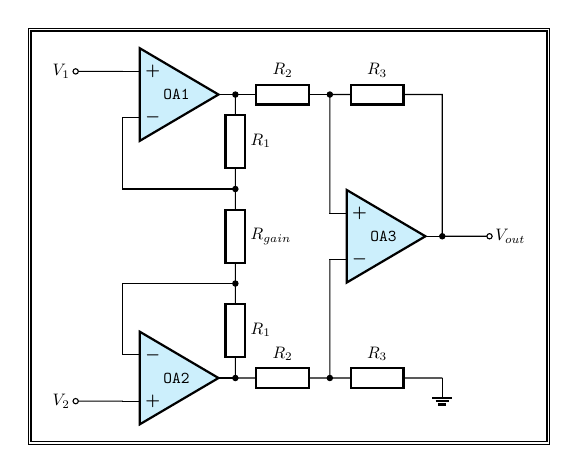
\begin{tikzpicture}[baseline={(current bounding box.center)}]
            \node{    
                \begin{circuitikz}[scale=\circuitsscale, transform shape, use fpu reciprocal]
                    \draw (0,0)
                        node[op amp, noinv input up, fill=cyan!20](OA1){\texttt{OA1}}
                        \opampPMCenter{OA1};
                    \draw (OA1.+) ++(-1,0)
                        node[left]{$V_1$}
                        to[short, o-] ++(1,0);
                    \draw (OA1.out)
                        to[short, -*] ++(0,0)
                        to[R, l=$R_1$, -*] ++(0,-2)
                        coordinate(OA1-R1Rg)
                        to[R, l=$R_{gain}$, -*] ++(0,-2)
                        coordinate(OA2-R1Rg)
                        to[R, l=$R_1$, -*] ++(0,-2)
                        node[op amp, fill=cyan!20, anchor=out](OA2){\texttt{OA2}};
                    \draw (OA2.+) ++(-1,0)
                        node[left]{$V_2$}
                        to[short, o-] ++(1,0);
                    \draw (OA1-R1Rg)
                        -- (OA1.- |- OA1-R1Rg)
                        -- (OA1.-);
                    \draw (OA2-R1Rg)
                        -- (OA2.- |- OA2-R1Rg)
                        -- (OA2.-);
                    \draw (OA1.out)
                        to[R, l=$R_2$, -*] ++(2,0)
                        coordinate(R2R3-up);
                    \draw (OA2.out)
                        to[R, l=$R_2$, -*] ++(2,0)
                        coordinate(R2R3-down);
                    \draw ($(R2R3-up)!.5!(R2R3-down)$) ++(opampPMCenter)
                        node[op amp, noinv input up, fill=cyan!20, anchor=center](OA3){\texttt{OA3}};
                    \draw (OA3.+)
                        -- (R2R3-up);
                    \draw (OA3.-)
                        -- (R2R3-down);
                    \draw (R2R3-up)
                        to[R, l=$R_3$] ++(2,0)
                        -- (OA3.out |- R2R3-up)
                        to[short, -*](OA3.out)
                        coordinate(OA3-Vout);
                    \draw (OA3.out) ++(1,0)
                        node[right]{$V_{out}$}
                        to[short, o-] ++(-1,0);
                    \draw (R2R3-down)
                        to[R, l=$R_3$] ++(2,0)
                        -- (OA3.out |- R2R3-down)
                        node[ground]{};
                \end{circuitikz}
                };

            \draw[black, double]
                (current bounding box.south west) ++(-\fboxsep, -\fboxsep) coordinate (ll)
                (current bounding box.north east) ++(\fboxsep, \fboxsep) coordinate (ur)
                (ll) rectangle (ur);
        \end{tikzpicture}
        \hspace*{\stretch{1.0}}
        $A_v=\frac{V_{out}}{V_2 + V_1}=\left(1+\frac{2 R_1}{R_{gain}}\right) \frac{R_3}{R_2}$
        \hspace*{\stretch{1.0}}
        \captionsetup{justification=centering}
        \caption{\small{INA's schematic and transfer function \parenciteit{}{INA:Wiki}, usually $R_1$, $R_2$, $R_3$ are built in the IC, and instead of $R_{gain}$ there are dedicated pins to connect it.}}
        \label{fig:INA}
    \end{figure}

    \subsection*{Circuit Diagram}
    \hspace{\parindent} The circuit as said in previous section, Filter topology and function, the circuit in Fig.%\ref{fig:CircDia}
    is subdivided in 4 stages: INA, HPF, LPF, PGA \& ADC

    \printbibheading
    \printbibliography[keyword=major, heading=subbibliography, title={Major Sources}]
    \printbibliography[keyword=minor, heading=subbibliography, title={Minor Sources}]
\end{document}